\documentclass[12pt]{article}
\usepackage[utf8]{inputenc}
\usepackage{mphysproject} % This includes graphicx, caption and geometry
\usepackage[block=space,bibencoding=utf8,style=phys,maxbibnames=6,giveninits=true]{biblatex}
\usepackage{amsmath}
\usepackage{physics}
\usepackage{siunitx}

\usepackage{hyperref}
\usepackage{cleveref}
\usepackage{float}
\usepackage{stackengine}
\usepackage{calc}
\usepackage{xcolor}

\usepackage[textsize=tiny]{todonotes}
\usepackage{lipsum}

\addbibresource{MPhys.bib}

\allowdisplaybreaks

% All kinds of mathy macros
\newcommand\textbff[1]{\textbf{\boldmath #1}}
\newcommand\circled[1]{\raisebox{.5pt}{\textcircled{\raisebox{-.9pt} {#1}}}
    }
\newcommand{\shortnote}[1]{\textit{\footnotesize (#1)}}

\newcommand{\pp}{\partial}
\newcommand{\mgrad}{\su{\nabla}}

% We often use underlines here
\stackMath
\newcommand\barbelow[1]{\stackunder[1pt]{#1}{\rule{\widthof{#1}*\real{1.1}}{.1ex}}}
\newcommand\twobarsbelow[1]{\stackunder[1pt]{\barbelow{#1}}{\rule{\widthof{#1}*\real{1.1}}{.1ex}}}
\newcommand{\su}[1]{\barbelow{#1}}
\newcommand{\du}[1]{\twobarsbelow{#1}}
\newcommand{\ssu}[1]{\scriptsize\barbelow{#1}\normalsize}
\newcommand{\sdu}[1]{\scriptsize\twobarsbelow{#1}\normalsize}

\newcommand{\QQ}{$\du{Q}$}
\newcommand{\NN}{$\su{N}$}
\newcommand{\EE}{$\du{E}$}
\newcommand{\PP}{$\du{\Pi}$}
\newcommand{\ddelta}[4]{\delta_{#1#3}\delta_{#2#4} + \delta_{#1#4}\delta_{#2#3}}

\newcommand{\onedot}{$\mathsurround0pt\ldotp$}
\newcommand{\cddot}{\mathbin{
    \vcenter{\baselineskip1ex \vspace{-0.1ex}\hbox{\onedot}\hbox{\onedot}}
}}

\begin{document}

\title{Normal Complex Tensor Order Parameter for Smectics in 3D}
\author{Jan Kocka}
\supervisor{Tyler N Shendruk}
%\date{1st January 2018}

\begin{abstract}
    \lipsum[10]
\end{abstract}

\maketitle

% This command introduces the Personal Statement: DO NOT REMOVE IT
\personalstatement
% Write PS here
\acknowledgments
% Write Acknowledgements here

\maintext

\section{Smectic Liquid Crystals}
\begin{figure}[t]
    \begin{center}
        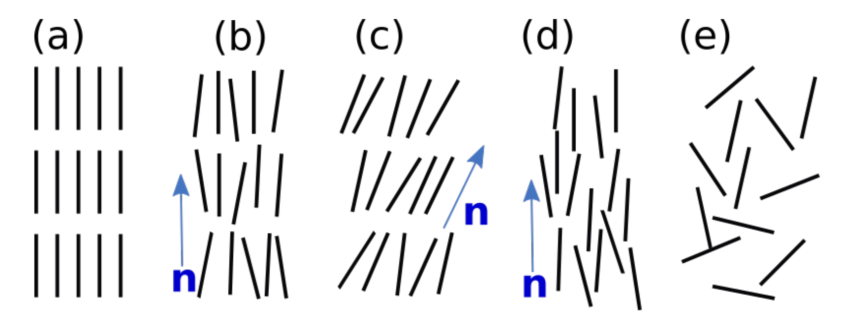
\includegraphics[width=0.95\textwidth]{figures/phases.pdf}
    \end{center}
    \caption{
        Illustrative structures of a substance made up from rod-like molecules.
        In order from (a) to (e) they are a fully crystalized phase, a smectic A, smectic C, nematic and an isotropic liquid.
    }\label{fig:phases}
\end{figure}
All physicists will be well familiar with the ordered crystalline phase, in which the relative positions and possibly orientation of molecules is ordered, predictable and often repeating.
Liquid crystals (LC) lay between this state and a typical liquid, some aspects of the phase are ordered, but others are not.
This is best illustrated as a transition from an unordered (isotropic) liquid state as in \cref{fig:phases}.

In an isotropic liquid the molecules have random, uncorrelated positions and orientations.
Note that we talk about orientations, these are naturally only present if the molecules themselves are not spherical/symmetric.
Depending on just how asymmetric they are they can have one or two orientation directions (in 3D), here we mainly look at rod-like molecules which have one, the axis of symmetry.
The first step in ordering is usually a transition to a nematic liquid crystal in which the orientations of nearby molecules align, see \cref{fig:phases}.
An important detail of nematic liquid crystals is that often the constituent molecules are symmetric along their length as well (the is no head and tail) as this changes the physics, a nematic phase which does not have this symmetry is called a polar nematic.

Next can come partial positional order, while different classification exist, in essence there are two ways this can happen in 3D.
Either the symmetry is broken along one axis, these are the smectic phases, or along two in the columnar phases\cite{oswaldNematicCholestericLiquid2005}.
In the columnar phases there remains only local one direction along which the system is not ordered.
As such these phases are composed of separated columns of flowing liquid which are at ordered positions much like a 2D crystal.
In the smectic phases, a broken symmetry along one axis results in a layered structure, the system is isotropic and flows within the layers but is organized along the layer normal.
As such, smectics are fundamentally a layered phase, and that is what we focus on in this project, in essence we create a mesoscopic model for layering.

There are various types of smectic phases, the simplest being the smectic A and C shown in \cref{fig:phases}.
It is worth pointing out that the smectic layering coexists with a nematic order of the molecules.
In smectic A phases the nematic orientation is always perpendicular to the layering, whereas in smectic C phases these are at an angle.
Besides these there is a class of hexatic smectic phases, in which the molecules within layers locally arrange in a hexagonal lattice.
However, while the lattice itself is only maintained for short distances, these local hexatic lattices have an orientation to them as well and this is aligned over large distances.
Thus these feature yet more order than the smectic A and C phases, they include the B$_\text{hex}$ phase which has the nematic director perpendicular to the layering, along with the F and I phases which have an angle between the two.
There are also smectic-like crystals which feature fully ordered often hexatic layers, among these are the B and E phases.
For more details on these structures see \cite{oswaldNematicCholestericLiquid2005,oswaldSmecticColumnarLiquid2005b,gennesPhysicsLiquidCrystals1995}.

\todo[inline,size=\footnotesize]{This could be extended pretty much indefinitely, given the twist data we have perhaps the TGB would be the next thing worth mentioning}
\todo[inline,size=\footnotesize]{Paragraph on why are they important/useful etc, the usual are soap, displays and hopefully something new? Bacteria! that might need a citation}

The model presented in this thesis is in its early stages and so we mainly aim to capture the physics of the A and perhaps C phases.
Though as we have extended the model into 3D it further highlighted that it captures the general concept of layers, and it does not currently have any concept of the underlying nematic order of smectics.
There is a way to add that and it is perhaps the next step in developing this theory, however it also shows that the model might be used in other fields which require a mesoscopic model for layering.
\todo{I don't like this paragraph but want to mention some of it somehow}

\subsection{Ginzburg-Landau theory and the nematic \QQ\ tensor}
Ginzburg-Landau theory is a powerful recipe to build phase transition theories, the work in this thesis being one of them.
As such we start by introducing these on the example of an isotropic liquid to nematic LC transition as there are many similarities to our smectic model.

The central concept of Ginzburg-Landau theory is the order parameter, this is usually some mathematical object such as a scalar, vector or tensor that has known values for each of the phases and varies in between them in mostly a smooth manner.
If a single order parameter is used to describe the entire system in question as a whole, it is a Landau theory, one can extract useful information using this alone.
However, Ginzburg-Landau theory goes a step further and promotes the order parameter to a field.
This way one may have a part of the system be in one phase and a different part in the other.

Going back to our example of a nematic LC, this order parameter needs to capture how aligned the molecules are at each point, accounting for the nematic symmetry.
The way to do this is using the \QQ\ tensor which can be obtained from a system of discrete molecules via
\begin{equation}
    \du{Q}_\text{mol} = \su{N}_\text{mol}\su{N}_\text{mol} - \frac{\du{\delta}}{d}
\end{equation}
where $\su{N}_\text{mol}$ is a unit vector denoting the orientation of a molecule, $\du{\delta}$ the identity and $d$ the dimensionality of the system (2 or 3).
Throughout this thesis, if two tensors appear side by side then it means a dyadic/tensor product and any contractions are denoted by dots \nolinebreak $\cdot$ (their order usually does not matter).
Note that $\du{Q}_\text{mol}$ immediately satisfies the nematic symmetry of to $\su{N}_\text{mol}$ being the same as $-\su{N}_\text{mol}$.
So each molecule has a $\du{Q}_\text{mol}$ and we take a local average of these to arrive at the tensor field \QQ\ (taking these local minima numerically can be quite tricky).
Given the form of \QQ\ we can then reexpress it as the following
\begin{equation}
    \du{Q} = S\qty(\su{N} \su{N} - \frac{\du{\delta}}{d}) \color{gray} + \text{possibly more terms, ignore for simplicity here} \normalcolor
\end{equation}
where $S$ is a number between 0 and 1 and $\su{N}$ is a unit vector.
From there it is easy to see that an isotropic liquid would have $\du{Q} = S = 0$ and a fully nematic one would have $S = 1$ and \NN\ be the orientation of the phase.
From this it is clear that $\du{Q}$ is a valid order parameter to describe the isotropic to nematic transition, it is in fact the most widely used such parameter due to it respecting the orientational symmetry.

Now that we have an order parameter, the next step in forming a Ginzburg-Landau theory is to find a suitable free energy functional.
This will be a volume integral of a free energy density $f(\su{r})$ over the system and potentially surface contributions, though often these are dealt with separately.
$f(\su{r})$ should only depend on the order parameter \QQ\ and elastic constants and crucially it must maintain any symmetries of the system.
This is where the power of Ginzburg-Landau theories lays as one does not have to derive these from microscopic interactions but may instead start taking all the possible terms of the order parameter that satisfy the system symmetries in increasing powers and stop when all the physics is captured.

% To do that one may look at the microscopic forces between individual molecules and coarse-grain these to a resulting 

\subsection{Biaxiality of \QQ}
There is one additional bit of complexity worth introducing and that is biaxiality of nematics.
We have been talking about the orientation of molecules as being a single direction, which is correct for rod-like molecules.
However, if the molecules are completely asymmetric then there can be order in two perpendicular directions.
Say we have long cuboid molecules, they can first order by aligning their longest axes and then also rotate around those axes so that the next longest axes also align.
The same applies to any asymmetrical shaped molecules in 3D.
It demonstrates the power of \QQ\ that we can still use it to decribe this dual order, we can still calculate it exactly the same way through $\du{Q}_\text{mol}$ and \QQ\ will still be symmetric and traceless, however it will now take the more general form
\begin{equation}
    \du{Q} = S_1\qty(\su{N} \su{N} - \frac{\du{\delta}}{d}) + S_2\qty(\su{M} \su{M} - \frac{\du{\delta}}{d})
\end{equation}
where $\su{N}$ and $\su{M}$ are mutually orthogonal unit vectors which describe the directions of the two orders, with $S_1$ and $S_2$ acting as their corresponding order parameters.

\subsection{Describing/modelling smectics\cite{oswaldSmecticColumnarLiquid2005b}}
Fundamentally, the layered positional order corresponds to a wave-like density fluctuation.
If we only consider a single wave throughout the system we have
\begin{equation}
    \rho(\su{r}) = \rho_0 + \rho_1\cos(\su{q_0}\cdot\su{r} + \phi) = \rho_0 + \Re(\rho_1 e^{i(\ssu{q_0} \cdot \ssu{r} + \phi)})
\end{equation}
where $\rho_0$ is the average density, $\rho_1$ is the wave amplitude, $\su{q_0}$ its wavevector containing both the wave direction and spacing and $\phi$ an arbitrary phase (determined by boundary conditions).

\subsection{The Problems\todo{also discuss Pevniy}}
\subsection{Other approaches and recent smecic results}

\section{Introduction to the \EE\ tensor}
We start by considering the density fluctuation as we have before
\begin{equation}
    \rho \simeq \rho_0 + 2\Re(\psi e^{i \ssu{q_0} \cdot \ssu{r}})
\end{equation}
but we allow the complex $\psi$ and the direction of $\su{q_0}$ both to be vary as fields leading to the wave part of the density being
\begin{equation}
    |\psi(\su{r})|e^{i (q_0 \ssu{N}(\ssu{r}) \cdot \ssu{r} + \phi(\ssu{r}))}
\end{equation}
with $q_0$ corresponding to the natural spacing of the wave.
Both $\su{N}$ and $\phi$ influence the phase, as before a constant gradient in $\phi$ corresponding to a constant contraction/dilation.


\section{New perspectives on \EE\ (in 3D)}
\subsection{Constraints}
\subsection{Biaxiality}
\subsection{Properties of biaxial \EE}
\begin{align}
    \du{E} &= \psi_1 (\su{N}\su{N} - \frac{\du{\delta}}{d}) + \psi_2 (\su{M}\su{M} - \frac{\du{\delta}}{d}) \\
    |\du{E}|^2 &= \du{E} \cddot \du{E}^* = (|\psi_1|^2 + |\psi_2|^2) (1 - 2 \frac{1}{d} + \frac{d}{d^2}) + (\psi_1\psi_2^* + \psi_1^*\psi_2) (-2\frac{1}{d} + \frac{d}{d^2}) \\
    &= \frac{d-1}{d} (|\psi_1|^2 + |\psi_2|^2) - \frac{1}{d} (\psi_1\psi_2^* + \psi_1^*\psi_2) \\
    &= (|\psi_1|^2 + |\psi_2|^2) - \frac{1}{d} (|\psi_1|^2 + |\psi_2|^2 + \psi_1\psi_2^* + \psi_1^*\psi_2) \\
    &= |\psi_1|^2 + |\psi_2|^2 - \frac{|\psi_1 + \psi_2|^2}{d} \\
    |\du{E_{eq}}|^2 &= \frac{d-1}{d}
\end{align}

\section{Dynamics of \EE}
\subsection{Ginzburg-Landau}
\subsection{Free Energy}

\begin{align}
    f_\text{bulk} = A |\du{E}|^2 - \frac{C}{2}|\du{E}|^4 \rightarrow |\du{E_{eq}}|^2 = \frac{A}{C}
\end{align}

\subsection{Projection operators}

\subsection{Taking the functional derivatives}

\section{Numerical considerations}
\subsection{Approximating \PP\todo{mention the sqrt thing! And the small E thing}}
\subsection{System boundaries \todo{mix of Dirichlet and von Neumann}}

\section{Numerical Results}
\subsection{Imposed twist}
\subsubsection{Fitting $\frac{\theta}{\Delta\theta}$}
We now want to quantify the shapes of the azimuthal angle $\theta$ as a function of height.
To do that, we first of all non-dimensionalize these quantities and instead look at $\frac{\theta}{\Delta\theta}$ as a function of $\frac{h}{H}$.
That way all the plots will have the same end points and so can be compared, notably these endpoints will be at $(0, 0)$ and $(1, 1)$ and by symmetry they also ought to go through $(\frac{1}{2}, \frac{1}{2})$.
Further as the shape is clearly a sigmoidal one, we attempted a fit using both the $\arctan$ and the $\tanh$ functions, both of which only leave one parameter once the endpoints are fixed.
As the $\arctan$ method performed qualitatively better (see \todo{do cref} for an example comparison of the two), we only use that from now on.
Its exact form is
\begin{equation}
    \frac{\theta}{\Delta\theta} = \frac{\arctan(a \qty(\frac{h}{H} - \frac{1}{2}))}{2\arctan(\frac{a}{2})} + \frac{1}{2}
\end{equation}
and we also quote that the slope of this function evaluated at $\frac{h}{H} = \frac{1}{2}$ is
\begin{equation}
    \eval{\dv{\frac{\theta}{\Delta\theta}}{\frac{h}{H}}}_\text{middle} = \frac{a}{2\arctan(\frac{a}{2})}
\end{equation}

\section{Current limitations of \EE}
\subsection{The smectic symmetries}
Earlier, in the motivational part of this thesis I have mentioned that one of the advantages of \EE\ is that it respects the symmetry of reversing the layering direction \NN\ both globally and locally.
While this is the true symmetry of a layered system, it is not a symmetry of the established relation between $|\psi|,\phi,\su{N}$ and the density modulation
\begin{equation}\label{eq:lim_den2}
    \rho(\su{r}) = \rho_0 + \Re(|\psi| e^{i(q_0\ssu{N}\cdot\ssu{r} + \phi)}), \qq{$|\psi|,\su{N}$ and $\phi$ being fields}
\end{equation}
which we did not directly use in this work, but it heavily guided our interpretation of the field.
The only symmetry of \cref{eq:lim_den2} is under simultaneously exchanging $\su{N}, \phi \leftrightarrow -\su{N}, -\phi$ locally or globally.
There are naturally two ways to resolve this issue.
Either modify \EE, in particular its complex phase, such that it respects the symmetry of \cref{eq:lim_den2}.
Or find a different way to interpret the fields from \EE\ as it is, or perhaps a combination of both approaches.

For modifying \EE, I suspect this would be very difficult to the point where any suitable form of \EE\ would likely be so different it should be called something else.
This is as one would need to somehow couple the complex phase $\phi$ and \NN, an eigenvector of \EE, which is only accessible numerically.
This is as the only symmetry of \cref{eq:lim_den2} is when the signs of both flip, not just one.
Regardless, if one was to find a form for \EE\ that satisfied both symmetries independently the interpretation of $\phi$ would not hold anymore.
Currently, using \cref{eq:lim_den2}, we interpret $\dv{\phi}{x}$ (with x being the direction along \NN\ at any point) as a contraction if it is positive and dilation if negative.
However, the change of $\phi \rightarrow -\phi$ will change the sign of these and so clearly this is not a physical symmetry of the system.

Thus, it seems the more natural way to move forward is to adapt \cref{eq:lim_den2} to respect the symmetry in \NN\ only.
Starting from a wave resembling $e^{i(\ssu{q_0}\cdot\ssu{r})}$ of which we want to adjust the wavelength locally.
Given the addition in \cref{eq:lim_den2} using $e^{i(\ssu{q_0}\cdot\ssu{r})(1+s(\ssu{r}))}$ might be a good starting point, where $s=0$ corresponds to equilibrium spacing, $s>1$ to a contraction and $s<1$ to a dilation.
This form has the required symmetry and can be expanded as
\begin{equation}
    e^{i(\ssu{q_0}\cdot\ssu{r})(1+s(\ssu{r}))} = e^{i(q_0\ssu{N}\cdot\ssu{r} + s(\ssu{r})q_0\ssu{N}\cdot\ssu{r})} 
\end{equation}
which now has the same form as \cref{eq:lim_den2} with $\phi(\su{r}) = s(\su{r})q_0\su{N}\cdot\su{r}$, however it is very important to stress that that would no longer be the $\phi$ from \EE\ as that would not change anything.
However, $s$ and $\phi$ from \EE\ are both dimensionless quantities and perhaps we can find a way to map them onto each other.
The only reasonable values for $s$ are from $-1$, where the wavelength becomes infinite, to $+\inf$ where wavelength goes to 0.
Any values $<-1$ would just correspond to a different $s$ and a flipped $\su{N}$.
On the other hand $\phi$ from \EE\ belongs to any set interval of length $2\pi$.
So if we use $\phi \in (-\pi, \pi]$ and let $s = \frac{\phi}{\pi}$ then the model could account for any dilation and a contraction of up to half the natural wavelength.
However, this would fundamentally change what $\phi$ from \EE\ is and would require more work to investigate any free energy costs to contractions and dilations, among other considerations.

\newpage
\printbibliography

\end{document}
